%	!Mode::"UTF-8"
%	本模板设置改自北京大学交叉学院 王宇哲学长和北京大学化学与分子工程学院 王应泽同学的分享,特此感谢!
%	模板制作:北京大学化学与分子工程学院 王梓涵
%	Email:2100011837@stu.pku.edu.cn
%	本模板仅适用于北京大学物理化学实验报告,其他学校请自行修改
%	吐槽:Latex用于写物化实验报告还是过于繁琐了,不过还是比Word好用多了(๑•̀ㅂ•́)و✧ (此吐槽由copilot自动生成,模板作者认为word更好用)
%	本模板仅供交流学习使用,不可用作商业用途。

\documentclass[12pt]{article}

%	页面设置
\usepackage{geometry}
\geometry{left=2.5cm, right=2.5cm, top=2.5cm, bottom=2.5cm}
\usepackage{graphicx}
\usepackage{ctex}
\usepackage{fontspec}
\usepackage{setspace}
\usepackage[usenames,dvipsnames]{xcolor}
\usepackage{titlesec}

%	字体设置
\setmainfont{Times New Roman}
\setCJKmainfont{SimSun}
\setCJKsansfont{SimHei}
\setCJKmainfont[AutoFakeBold=true]{SimSun}

%	表格设置\
\usepackage{array,colortbl}
\usepackage{makecell}
\newcommand{\addcell}[2][4]{\makecell{\zihao{#1}\textsf{#2}}}
\usepackage{titlesec}
\usepackage{booktabs}
\usepackage{ragged2e} 
\usepackage{multirow}
\usepackage{tabularx}

% 网址设置
\usepackage{hyperref}
\hypersetup{hidelinks,
	colorlinks=true,
	allcolors=black,
	pdfstartview=Fit,
	breaklinks=true}


%	设置图注、表注
\usepackage{caption}
\usepackage{bicaption}
\captionsetup{labelsep=quad, font={small, bf}, skip=2pt}
\DeclareCaptionOption{english}[]{
    \renewcommand\figurename{Fig.}
    \renewcommand\tablename{Table}
}
\captionsetup[bi-second]{english}

%	设置页眉
\usepackage{fancyhdr}
\usepackage{xpatch}
\pagestyle{fancy}
\fancypagestyle{preContent}{
    	\fancyhead[L]{\zihao{-5} 物理化学实验}
    	\fancyhead[C]{\zihao{-5} 实验五\ \ 双液体系沸点-成分图的绘制}
    	\fancyhead[R]{\zihao{-5} 2100011837\ 王梓涵}
		\renewcommand{\headrulewidth}{2pt}
		\renewcommand{\footrulewidth}{1pt}
		\xpretocmd\headrule{\color{BrickRed}}{}{\PatchFailed} % 设置页眉分割线颜色
		\xpretocmd\footrule{\color{BrickRed}}{}{\PatchFailed} % 设置页脚分割线颜色
}
\pagestyle{preContent}



%	设置首页页眉及取消首页页脚 若不需要首页页眉 请注释掉下列内容
\fancypagestyle{plain}{
	\fancyhead[L]{\zihao{-5} 物理化学实验}
    \fancyhead[C]{\zihao{-5} 实验五\ \ 双液体系沸点-成分图的绘制}
	\fancyhead[R]{\zihao{-5} 2100011837\ 王梓涵}
	\cfoot{}
}

%	设置标题格式
\titleformat*{\section}{\color{Mahogany}\zihao{4}\sffamily}
\titleformat*{\subsection}{\zihao{-4}\sffamily}
\titleformat*{\subsubsection}{\zihao{-4}\sffamily}
\titlespacing*{\section}{0pt}{10pt}{10pt}
\titlespacing*{\subsection}{0pt}{10pt}{5pt}
\titlespacing*{\subsubsection}{0pt}{10pt}{5pt}


%	设置引用格式(ACS格式规范)
%	注意:请安装JabRef
%	JabRef使用参考:https://blog.csdn.net/weixin_44191286/article/details/85698921
\usepackage[super,round,comma,compress]{natbib}

%	数学公式增强
\usepackage{amsmath}
\usepackage{amssymb}

%	单位与数学式
\usepackage{siunitx}

% 其他添加
\usepackage[version=4]{mhchem}

%	设置封面
\begin{document}
    % 标题页
    \begin{titlepage}
    	% 页眉
    	\thispagestyle{plain}
        % 校徽图片
        \begin{figure}[h]
            \centering
            \includegraphics{pku.png}
        \end{figure}
        \vspace{24pt}
        % 标题
        \centerline{\zihao{-0} \textsf{\textcolor{Mahogany}{物理化学实验报告}}}
        \vspace{40pt} % 空行
        \begin{center}
            \begin{tabular}{cp{14.1cm}}
                % 题目
                \addcell[2]{题目:} & \addcell[1]{双液体系沸点-成分图的绘制} \\
                \cline{2-2}
            \end{tabular}
        \end{center}
        \vspace{20pt} % 空行
        \begin{center}
            \doublespacing
            \begin{tabular}{cp{5cm}}
                % 姓名
                \addcell{姓\phantom{空格}名:\ } & \addcell{王梓涵} \\
                \cline{2-2}
                % 学号
                \addcell{学\phantom{空格}号:\ } & \addcell{2100011837}\\
                \cline{2-2}
                % 组别
                \addcell{组\phantom{空格}别:\ } & \addcell{22组} \\
                \cline{2-2}
                % 实验日期
                \addcell{实验日期:\ } & \addcell{2023.11.23}\\
                \cline{2-2}
                % 室温
                \addcell{室\phantom{空格}温:\ } & \addcell{292.85\ K}\\
                \cline{2-2}
                % 大气压强
                \addcell{大气压强:\ } & \addcell{102.38\ kPa}\\
                \cline{2-2}
            \end{tabular}
            \begin{tabular*}{\textwidth}{c}
                \\ % 这是空行
                \\ % 这是空行
                \\ % 这是空行
                \hline % 分割线
            \end{tabular*}
        \end{center}
        % 摘要
        \textsf{\textcolor{BrickRed}{摘\ \ 要}}\ \  \  本实验测量了一系列乙醇-环己烷标准溶液的折射率,作出了乙醇质量分数$x$乙醇与折射率$n$的标准工作曲线。通过回流冷凝法测定了不同浓度乙醇-环己烷体系的沸点和气相、液相折射率,计算了各平衡沸点下的两相组成,绘制了乙醇-环己烷体系沸点-成分图,确定了恒沸点$t_{b}=65.03\sim 65.45\ \ {\rm ^{\circ}C}$,组成为$\chi_{\ce{EtOH}}=0.307 \sim 0.310$。讨论了此实验可能引入误差的位置并讨论了改进方案。
        \\
        \\
        % 关键字
        \textsf{\textcolor{BrickRed}{关键词}}\ \ \  乙醇-环己烷体系,沸点-成分图,回流冷凝法,折射率,工作曲线
    \end{titlepage}

    \section{引言}
		\subsection{实验目的}
			本实验的实验目的主要有以下几点\citealp{physchemlab}:\par
			\ \ \ \ \ \ \ \ 1. 测定不同浓厚的环己烷-乙醇体系的沸点和气、液两项的平衡成分。\par
			\ \ \ \ \ \ \ \	2. 绘制沸点-成分图,并确定体系的最低恒沸点和组成。\par
			\ \ \ \ \ \ \ \	3. 掌握阿贝折射仪的使用方法。\par

		\par
			\subsection{实验原理和实验方法}
				实验原理和实验方法在实验预习报告中如\textbf{图1}所示: \par
		\begin{figure}[h]
			\centering
			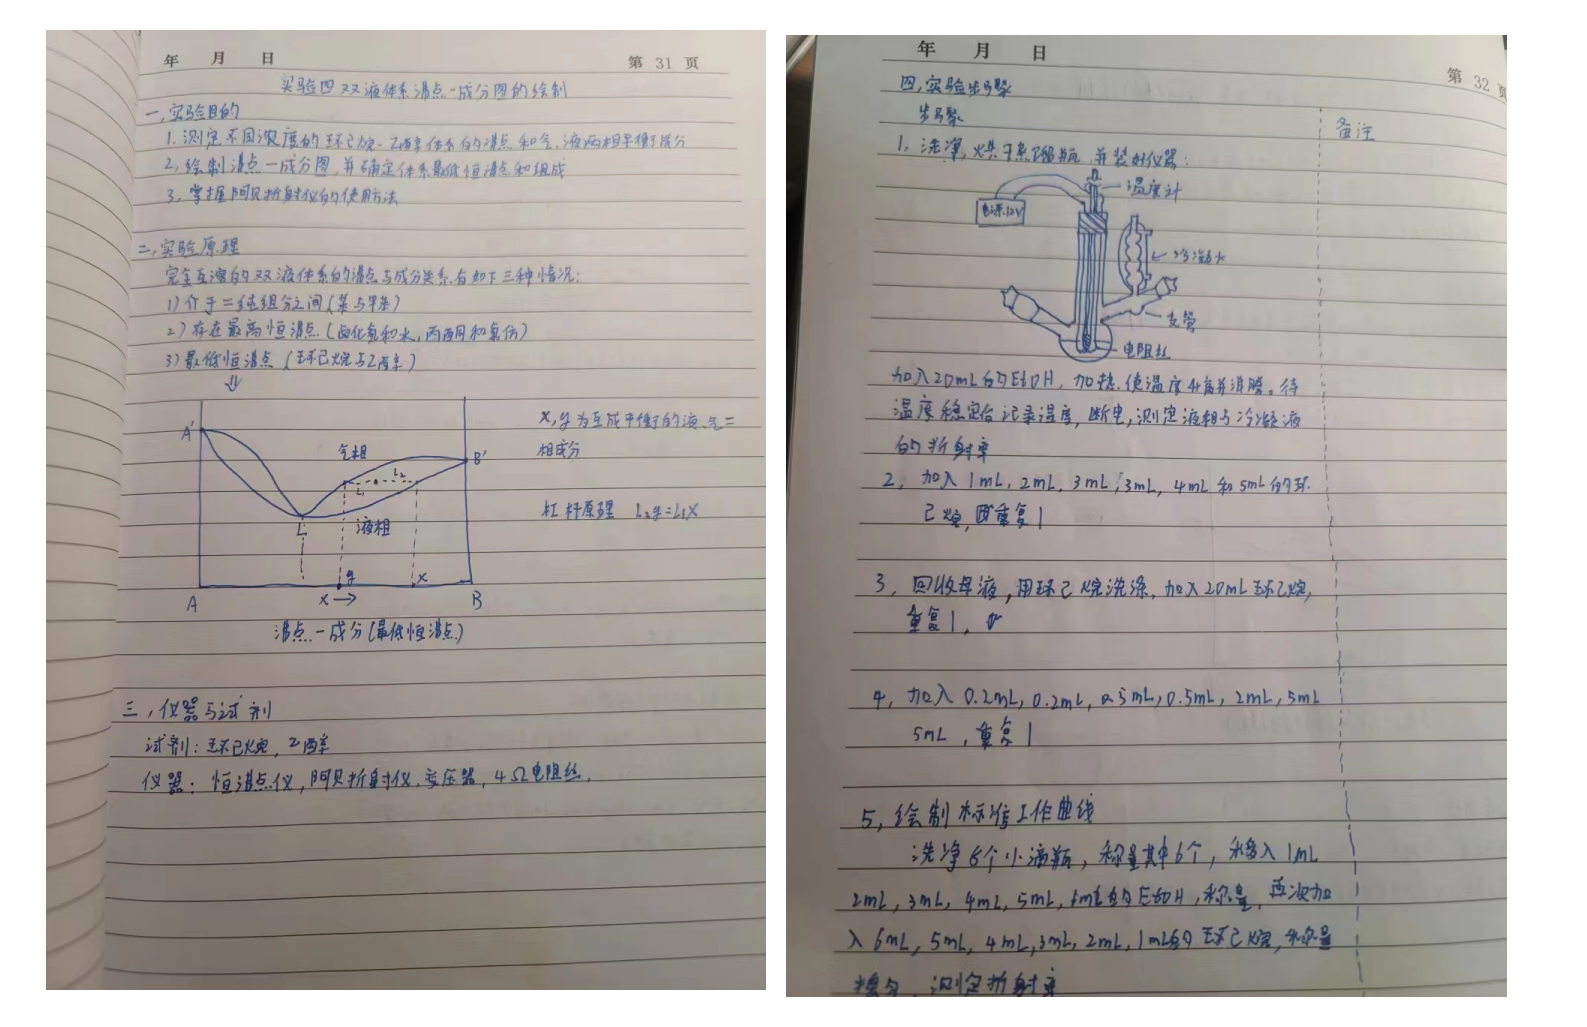
\includegraphics[width=0.9\textwidth]{1.png}
			\bicaption{实验预习报告的实验原理部分}{The principle part of the experiment in the experiment preview report}
		\end{figure}

	     
    \section{实验部分}

    	\subsection{仪器和试剂}
    		\textbf{仪器}:\ \  恒沸点仪,阿贝折射仪,变压器,$4\ \ \Omega$电阻丝,$1/10$刻度温度计,试管,小滴瓶,$1\ \ {\rm mL}$移液管,$5\ \ {\rm mL}$移液管,$20\ \ {\rm mL}$移液管,蒸馏烧瓶。\par
			\textbf{试剂}:\ \  环己烷(AR),乙醇(AR);

    	\subsection{实验内容\citealp{physchemlab}}
			本实验的实验操作如下所示,其中笔者的思考和具体实验中的不同操作会在括号中写出。\par
			\subsubsection{测量纯乙醇和环己烷的折射率}
				用丙酮清洗阿贝折射仪的,调节使得明暗交界面清晰。分别滴加AR乙醇和AR环己烷,测量其折射率。 \par
			\subsubsection{测量纯乙醇和沸点和气、液折射率}
				按照\textbf{图2}装好仪器,温度计的水银球$1/2$浸入液体内,冷凝管内通入冷水。将电阻丝接在输出电压$12.6\ \ {\rm V}$的变压器上,使温度升高并沸腾。待温度稳定后数分钟,记下温度及大气压。切断电源,用两支干净的滴管,分别取出支管处的气相冷凝液和蒸馏瓶中的液体几滴,使用阿贝折射仪测定其折射率。\par
				\begin{figure}[h]
					\centering
					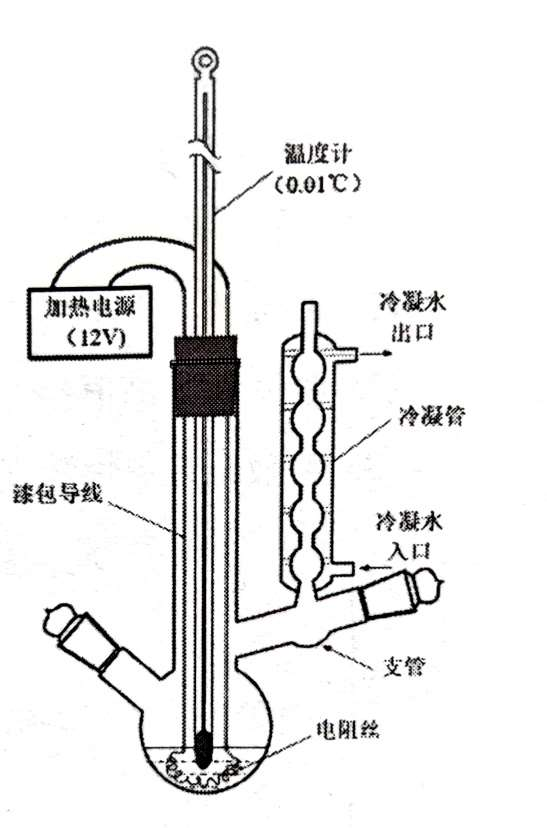
\includegraphics[width=0.3\textwidth]{2.png}
					\bicaption{实验室自制恒沸点仪}{Laboratory self-made constant boiling point instrument}
				\end{figure}
			
			\subsubsection{沸点和两相成分的测定}
				沿用\textbf{2.2.2}中的体系,向蒸馏瓶中加入$1\ \ {\rm mL}$环己烷,按\textbf{2.2.2}中方法测定平衡沸点$t_{b}$及气相折射率$n^{g}$、液相折射率$n^{l}$(\textbf{与2.2.2不同,混合体系测量折射率一定要快。因为在测量温度下环己烷的挥发要快于乙醇,这会导致测量过程中折射率会逐步减小,即向乙醇靠近。本人实测,以1:1的乙醇/环己烷为例,每隔30s折射率数值下降约0.05}) 。测量完成后再依次加入$1.00\ \ {\rm mL}$、$2.00\ \ {\rm mL}$、$3.00\ \ {\rm mL}$、$3.00\ \ {\rm mL}$、$4.00\ \ {\rm mL}$、$5.00\ \ {\rm mL}$环己烷,记录液体组成,进行同样的实验。\par
				上述实验结束后,回收母液,再用少量环己烷洗$3\sim 4$次蒸馏瓶,注入$20.00\ \ {\rm mL}$环己烷,再装好仪器。先测定纯环己烷的沸点,然后依次加入$0.20\ \ {\rm mL}$、$0.20\ \ {\rm mL}$、$0.50\ \ {\rm mL}$、$0.50\ \ {\rm mL}$、$2.00\ \ {\rm mL}$、$2.00\ \ {\rm mL}$、$5.00\ \ {\rm mL}$、$5.00\ \ {\rm mL}$乙醇,分别测定平衡沸点$t_{b}$及气相折射率$n^{g}$、液相折射率$n^{l}$。
			\subsubsection{标准工作曲线绘制}
				洗净并烘干$6$个小滴瓶,冷却后准确称量其质量$m_{0}$。用带刻度的移液管分别加入$1.00\ \ {\rm mL}$、$2.00\ \ {\rm mL}$、$3.00\ \ {\rm mL}$、$4.00\ \ {\rm mL}$、$5.00\ \ {\rm mL}$、$6.00\ \ {\rm mL}$、$7.00\ \ {\rm mL}$、$8.00\ \ {\rm mL}$乙醇,分别称量其质量$m_{1}$,再依次分别加入$8.00\ \ {\rm mL}$、$7.00\ \ {\rm mL}$、$6.00\ \ {\rm mL}$、$5.00\ \ {\rm mL}$、$4.00\ \ {\rm mL}$、$3.00\ \ {\rm mL}$、$2.00\ \ {\rm mL}$、$1.00\ \ {\rm mL}$环己烷,再分别称量其质量$m_{2}$,旋紧盖子后摇匀。在恒温$t=30.0\ \ {\rm ^{\circ}C}$下分别测定这些样品的折射率$n$。(\textbf{在实际过程中,溶剂会由整个小组的同学共同配置,本人配置的溶液为乙醇/环己烷=2:7的溶液。为保证测量平行性,每人会分别用自己台面上的折射仪测量折射率})\par 
				

	 \section{数据与结果}
 		\subsection{实验数据处理与分析}
 			\subsubsection{标准工作曲线的绘制}
			 记录加入乙醇体积$V_{\rm EtOH}$、加入环己烷体积$V_{Cy}$,称量小滴瓶空瓶质量$m_{0}$、加入乙醇后质量$m_{1}$、加入环己烷后质量$m_{2}$。宜春的质量分数可由下式计算得到:\par
			 $$
			 \chi_{\ce{EtOH}}=\frac{m_{1}-m_{0}}{m_{2}-m_{0}}
			 $$
			 在恒温$t=30.0\ \ {\rm ^{\circ}C}$下分别测定这些样品及纯乙醇、纯环己烷的折光率$n$,结果如\textbf{表1}所示:\par
			 \begin{table}[h]
				\arrayrulecolor{Maroon}
				 \centering
				 \zihao{5}
				 \bicaption{不同浓度乙醇-环己烷溶液的配制及折射率测定实验数据}{Preparation of EtOH-Cy solution and experimental data of refractive index}
				 \begin{tabular}{cccccccc}
					 \toprule
					 编号 & $V_{\rm EtOH}/{\rm mL}$ & $V_{\rm EtOH}/{\rm mL}$ & $m_{0}/{\rm g}$ &$m_{1}/{\rm g}$&$m_{2}/{\rm g}$& $\chi_{\ce{EtOH}}$&$n$ \\
					 \midrule
					 纯$\rm Cy$ &      &      &         &         &         & 0.0000 & 1.4209 \\
					 1     		& 1.00 & 8.00 & 28.5609 & 29.3394 & 35.5132 & 0.1120 & 1.4127 \\
					 2     		& 2.00 & 7.00 & 28.8807 & 30.4609 & 35.8635 & 0.2263 & 1.4040 \\
					 3     		& 3.00 & 6.00 & 33.1372 & 35.4767 & 40.1103 & 0.3355 & 1.3960 \\
					 4     		& 4.00 & 5.00 & 35.5170 & 38.6509 & 42.4492 & 0.4521 & 1.3881 \\
					 5     		& 5.00 & 4.00 & 27.3235 & 31.2277 & 34.3287 & 0.5573 & 1.3805 \\
					 6     		& 6.00 & 3.00 & 32.6557 & 37.3339 & 39.6379 & 0.6700 & 1.3734 \\
					 7     		& 7.00 & 2.00 & 32.1465 & 37.6582 & 39.2040 & 0.7810 & 1.3676 \\
					 8     		& 8.00 & 1.00 & 32.3848 & 38.6301 & 39.3847 & 0.8922 & 1.3627 \\
					 纯${\rm EtOH}$ &  &      &         &         &         & 1.0000 & 1.3575\\
					 \bottomrule
				 \end{tabular}
			 \end{table}
			 \par

			 根据\textbf{表1}数据,作出$n-\chi_{\ce{EtOH}}$关系的散点图,并用origin进行二次拟合(\textbf{不使用线性拟合的合理性将在实验讨论部分分析}),作出乙醇-环己烷体系的$n-\chi_{\ce{EtOH}}$工作曲线,如\textbf{图3}所示。\par
			\begin{figure}[!h]
				\centering
				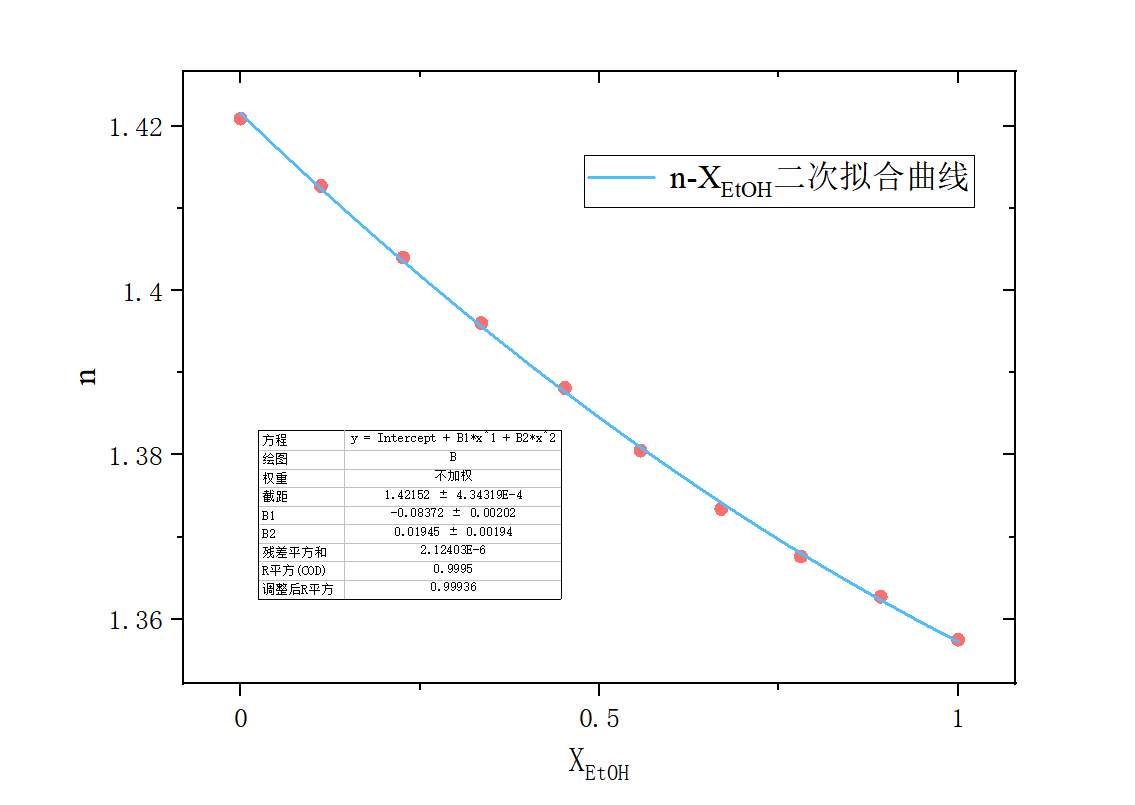
\includegraphics[width=0.70\textwidth]{3.png}
				\bicaption{乙醇-环己烷体系$n-\chi_{\ce{EtOH}}$标准工作曲线}{$n-\chi_{\ce{EtOH}}$ Standard working curve of ethanol-cyclohexane system}
			\end{figure}
			得到的拟合曲线的方程为:
			$$
 			n=(0.01945\pm 0.002)\chi^{2}_{\ce{EtOH}}-(0.084\pm 0.002)\chi_{\ce{EtOH}}+(1.4215\pm 0.0004),\  \ R^{2}=0.99936
			$$
			\par
			根据\textbf{图3}可以看出,二次函数拟合得到$n-X_{\rm EtOH}$工作曲线收到了很好的效果,各个数据点
			基本落在拟合曲线上,因此可以作为可靠的工作曲线使用。

	 		\subsubsection{乙醇-环己烷溶液沸点及其两相折射率的测量}
			先测定乙醇中加入环己烷体系的平衡沸点$t_{b}$及气相折射率$n^{g}$、液相折射率$n^{l}$,记录液体的组成,记录于\textbf{表2}。上述实验结束后,回收母液,再用少量环己烷洗$3\sim 4$次蒸馏瓶,注入$20.00\ \ {\rm mL}$环己烷,再装好仪器。先测定纯环己烷的沸点,再分别测定加入不同量乙醇后的平衡沸点$t_{b}$及气相折射率$n^{g}$、液相折射率$n^{l}$,同样记录于\textbf{表2}中。\par
			对于每种组成的体系,气相和液相分别平行测量三次,其平均值$\bar{n_{l}}$和$\bar{n_{g}}$计算如下:\par
			$$
			\bar{n_{l}}=\frac{1}{3}\sum_{i=1}^{3}n^{l}_{i}
			$$
			$$
			\bar{n_{g}}=\frac{1}{3}\sum_{i=1}^{3}n^{g}_{i}
			$$
			得到的结果如\textbf{表2}所示。\par
			\begin{table}[h]
				\arrayrulecolor{Maroon}
				 \centering
				 \zihao{5}
				 \bicaption{不同浓度乙醇-环己烷溶液的配制及折射率测定实验数据}{Preparation of EtOH-Cy solution and experimental data of refractive index}
				 \begin{tabular}{cccccccccccc}
					 \toprule
					 编号 & $V_{\rm EtOH}/{\rm mL}$ & $V_{\rm EtOH}/{\rm mL}$ & $T_{b}/{\rm ^{\circ}C}$ &$n^{g}_{1}$&$n^{g}_{2}$& $n^{g}_{3}$&$n^{l}_{1}$&$n^{l}_{2}$&$n^{l}_{3}$&$\bar{n_{l}}$&$\bar{n_{g}}$ \\
					 \midrule
					 0 & 20   & 0  & 78.42 & 1.3569 & 1.3570 & 1.3569 & 1.3575 & 1.3575 & 1.3574 & 1.3575 & 1.3569 \\
					 1 & 20   & 1  & 75.93 & 1.3699 & 1.3697 & 1.3691 & 1.3595 & 1.3595 & 1.3595 & 1.3595 & 1.3696 \\
					 2 & 20   & 2  & 74.05 & 1.3766 & 1.3765 & 1.3764 & 1.3610 & 1.3611 & 1.3607 & 1.3609 & 1.3765 \\
					 3 & 20   & 4  & 73.02 & 1.3784 & 1.3886 & 1.3812 & 1.3653 & 1.3650 & 1.3653 & 1.3652 & 1.3827 \\
					 4 & 20   & 7  & 68.79 & 1.3920 & 1.3925 & 1.3925 & 1.3680 & 1.3690 & 1.3687 & 1.3686 & 1.3923 \\
					 5 & 20   & 10 & 66.79 & 1.3945 & 1.3950 & 1.3940 & 1.3745 & 1.3745 & 1.3740 & 1.3743 & 1.3945 \\
					 6 & 20   & 14 & 65.84 & 1.3950 & 1.3960 & 1.3965 & 1.3800 & 1.3805 & 1.3810 & 1.3805 & 1.3958 \\
					 7 & 20   & 19 & 65.60 & 1.3973 & 1.3978 & $-$    & 1.3865 & 1.3866 & 1.3870 & 1.3867 & 0.9317 \\
					   &      &    &       &        &        &        &        &        &        &        &        \\
					 0 & 0    & 20 & 80.85 & 1.4209 & 1.4209 & 1.4209 & 1.4210 & 1.4209 & 1.4209 & 1.4209 & 1.4209 \\
					 1 & 0.2  & 20 & 78.37 & 1.4080 & 1.4085 & $-$    & 1.4208 & 1.4208 & 1.4208 & 1.4208 & 0.9388 \\
					 2 & 0.4  & 20 & 75.52 & 1.4030 & 1.4029 & $-$    & 1.4199 & 1.4199 & 1.4197 & 1.4198 & 0.9353 \\
					 3 & 0.9  & 20 & 68.7  & 1.4000 & 1.3997 & 1.4001 & 1.4190 & 1.4187 & 1.4192 & 1.4190 & 1.3999 \\
					 4 & 1.4  & 20 & 66.86 & 1.3994 & 1.3990 & 1.3997 & 1.4160 & 1.4165 & 1.4163 & 1.4163 & 1.3994 \\
					 5 & 3.4  & 20 & 65.48 & 1.3984 & 1.3985 & 1.3980 & 1.4080 & 1.4085 & 1.4080 & 1.4082 & 1.3983 \\
					 6 & 8.4  & 20 & 65.23 & 1.3975 & 1.3974 & 1.3980 & 1.3974 & 1.3974 & 1.3975 & 1.3974 & 1.3976 \\
					 7 & 14.4 & 20 & 65.44 & 1.3968 & 1.3970 & 1.3975 & 1.3892 & 1.3895 & 1.3893 & 1.3893 & 1.3971 \\
					\bottomrule
				 \end{tabular}
			\end{table}
			\par
			可以注意到,其中部分气相数据并未平行记录三次,其原因由以下两点:\par
			\begin{enumerate}
				\item \textbf{液相量不足}:在实际测量过程中,气相收集的液体较少,因此有时收集的液体不足以测量三次。\par
				\item \textbf{最后一组数值不准}:为了尽快完成实验,实验者会在温度降至约50$^{\circ}C$时就开始取气相进行测量,这会导致气相中的环己烷快速挥发,导致第三个点测量的值偏离较大。\par
			\end{enumerate}
		\subsection{数据处理结果与分析}
			\subsubsection{气液平衡时液相、气相组成计算}
				根据\textbf{图3}二次函数插值得到的$n-\chi_{\ce{EtOH}}$标准工作曲线,将\textbf{表2}中的液相折射率$\bar{n_{l}}$、气相折射率$\bar{n_{g}}$换算成对应的液相中乙醇质量分数$\chi^{l}_{\ce{EtOH}}$、气相中乙醇质量分数$\chi^{g}_{\ce{EtOH}}$,结果如\textbf{表3}所示。
				\begin{table}[h]
					\centering
					\zihao{5}
					\bicaption{乙醇-环己烷体系气液平衡时液相、气相组成计算数据}{Calculation data of liquid and gas phase composition of EtOH-Cy at gas-liquid equilibrium}
					\begin{tabular}{cccccc}
						\toprule
						编号 & $t_{b}/{\rm ^{\circ}C}$ & $\bar{n_{l}}$ & $\chi^{l}_{\rm EtOH}$ &  $\bar{n_{g}}$& $\chi^{g}_{\ce{EtOH}}$ \\
						\midrule
						0 & 78.42 & 1.3575 & 1.000   & 1.3569 & 1.000  \\
						1 & 75.93 & 1.3595 & 0.9120 & 1.3696 & 0.7252 \\
						2 & 74.05 & 1.3609 & 0.8838 & 1.3765 & 0.6092 \\
						3 & 73.02 & 1.3652 & 0.8032 & 1.3827 & 0.5116 \\
						4 & 68.79 & 1.3686 & 0.7427 & 1.3923 & 0.3716  \\
						5 & 66.79 & 1.3743 & 0.6445 & 1.3945 & 0.3414 \\
						6 & 65.84 & 1.3805 & 0.5459 & 1.3958 & 0.3231 \\
						7 & 65.60 & 1.3867 & 0.4524 & 1.3976 & 0.2998 \\
						  &       &        &             &        &     \\
						0 & 80.85 & 1.4209 & 0.000    & 1.4209 & 0.000  \\
						1 & 78.37 & 1.4208 & 0.0082 & 1.4083 & 0.1604 \\
						2 & 75.52 & 1.4198 & 0.0195 & 1.4030 & 0.2282 \\
						3 & 68.7  & 1.4190 & 0.0298 & 1.3999 & 0.2679 \\
						4 & 66.86 & 1.4163 & 0.0619 & 1.3994 & 0.2754 \\
						5 & 65.48 & 1.4082 & 0.1615 & 1.3983 & 0.2897 \\
						6 & 65.23 & 1.3974 & 0.3014 & 1.3976 & 0.2987 \\
						7 & 65.44 & 1.3893 & 0.4142 & 1.3971 & 0.3059 \\	
						\bottomrule
					\end{tabular}
				\end{table}
				\par

				\subsubsection{乙醇-环己烷体系沸点-气、液成分图}
				近似认为实验过程中大气压恒为$p=102.38\ \ {\rm kPa}$,溶液沸点在恒定压强下测得。根据\textbf{表3}数据,以气相、液相中乙醇质量分数$\chi_{\ce{EtOH}}$为横坐标,平衡沸点$t_{b}$为纵坐标,绘制乙醇-环己烷体系的沸点-成分图,如\textbf{图4}所示。\par
				根据\textbf{图4},读出乙醇-环己烷体系的恒沸点为$t_{b}=65.03\sim 65.45\ \ {\rm ^{\circ}C}$,组成为$\chi_{\ce{EtOH}}=0.307 \sim 0.310$。查阅\textit{CRC Handbook of Chemistry and Physics}\citealp{crc},知乙醇-环己烷体系在近常压$p_{0}=102.26\ \ {\rm kPa}$下的恒沸点为$T_{b}=337.95\ \ {\rm K}$即$t_{b}=64.80\ \ {\rm ^{\circ}C}$,质量分数为$\chi_{\ce{EtOH}}=0.3128$。\par
				\begin{figure}[!h]
					\centering
					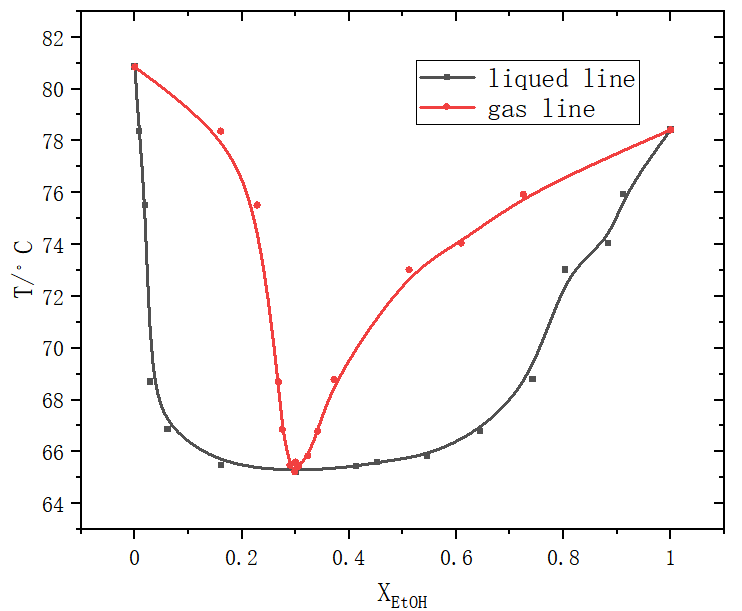
\includegraphics[width=0.65\textwidth]{4.png}
					\bicaption{乙醇-环己烷体系沸点-气、液成分图}{Boiling point-gas and liquid phase composition diagram of ethanol-cyclohexane system}
				\end{figure}
				\par
				可见实验测得乙醇-环己烷体系的恒沸点与组成均与文献参考值接近,说明实验测量结果较为可靠。\par

					\section{讨论与结论}
					\subsection{实验讨论}
					\subsubsection{标准工作曲线的拟合方式}
					在文中,实验者使用了使用二次函数插值作出乙醇-环己烷体系的$n-\chi_{\ce{EtOH}}$工作曲线,而非线性曲线。这里将结合理论推导作一简要分析为什么$n-\chi_{\ce{EtOH}}$标准工作曲线不具有线性的形式。\par 
					查阅文献可知\citealp{wenxian2},在一定温度下,物质的折射率$n$与摩尔浓度$c$呈线性关系,即:
					$$
					n=kc+A
					$$
					其中,理论上$A=1$,$k$为与入射光波长$\lambda$及物质本身性质有关的常数。假设实验中实际的乙醇-环己烷体系仅由乙醇、环己烷两相组成,则理论上的折射率为:
					$$
					n=k_{1}c_{EtOH}+k_{2}c_{Cy}+A
					$$ 		
					因$k_{1}$、$k_{2}$仅与物质自身的性质相关,而$c_{Cy}$与$c_{EtOH}$受到偏摩尔体积的影响,随两种组分的比例变化而变化,无法使用一个确切的函数描述。可由下式表示:
					$$
					c_{Cy}=\frac{n_{Cy}}{n_{Cy}(\frac{\partial V}{\partial n})_{n,T,P}+n_{EtOH}(\frac{\partial V}{\partial n})_{n,T,P}}
					$$
					若以摩尔分数$x_{Cy}$表示则有:
					$$
					c_{Cy}=\frac{x_{Cy}}{x_{Cy}(\frac{\partial V}{\partial n})_{n,T,P}+(1-x_{Cy})(\frac{\partial V}{\partial n})_{n,T,P}}
					$$
					此曲线为一个凸函数,无法用线性函数拟合,因此实验者使用二次函数拟合。\par
					\subsubsection{体系难以平衡}
					在实验过程中,实验者发现乙醇-环己烷体系很难达到平衡,体系的温度呈现阶梯状上升,而且再接近平衡温度时会有一定幅度的波动。产生这一现象的原因可能是由于加热用的电阻丝位于蒸馏烧瓶底部,且整个系统保温较差,蒸馏烧瓶内存在自下而上的温度梯度,靠近电阻丝的部分温度较高,而远离电阻丝的冷凝管处温度显著较低,且冷凝管内也存在自下而上的温度梯度,产生了一定的分馏现象。\par 
					同时为了接取气相组分,液体在回流时会先在凹陷处汇聚。由此形成液滴的表面张力会阻止液体顺畅的回流,使得体系长时间处于介稳态无法真正达到平衡。\par
					\subsection{误差讨论}
					笔者认为本次实验中误差可能来源于以下几个方面:
					\subsubsection{环己烷的快速挥发}
					在实验过程中,环己烷的挥发速率远大于乙醇,因此在测量过程中,环己烷的挥发会导致体系中环己烷的浓度逐渐降低,从而导致测量的折射率偏小。为了探究此挥发到底对结果影响有多大,实验者在等待蒸发体系平衡的间隙进行了实验,步骤如下:\par
					1. 利用废液缸配置浓度约为1:1的乙醇/环己烷溶液。\par
					2. 将溶液滴于阿贝折射仪上,使其暴露在空气中,经过不同的时间间隔后,测量其折射率。\par
					实验结果如\textbf{表4}所示。\par
					\begin{table}[h]
						\centering
						\zihao{5}
						\bicaption{乙醇-环己烷溶液在空气中的折射率变化}{Refractive index change of ethanol-cyclohexane solution in air}
						\begin{tabular}{ccc}
							\toprule
							序号& 时间$T/{\rm s}$ & 折射率$n$ \\
							\midrule
							1&0-5(立即测量)& 1.3855 \\
							2&10 & 1.3790  \\
							3&20 & 1.3733  \\
							4&30 & 1.3704  \\
							5&60 & 溶液干了  \\
							\bottomrule
						\end{tabular}
					\end{table}
					\par
					可以注意到,随着时间的增加,溶液的折射率逐渐降低,这说明环己烷的挥发确实会导致溶液的折射率降低,从而导致实验结果偏小。在实际操作中,若认为取溶液的时间平均为10s则其引入的误差为:\par
					$$
					\Delta n=\frac{1.3855-1.3790}{1.3855}=4.7\%
					$$
					考虑到试剂取溶液时温度更高,引入的误差可能更大。\par
					\subsubsection{取溶剂时的温度降低}
					在实验过程中,实验者会在温度降至约50$^{\circ}C$时就开始取气相进行测量,这回破坏原有的气液平衡,使得液相组分发生变化,从而引入误差。\par
					但考虑到本实验装置中气相的体积较小,根据理想气体状态方程:
					$$
					pV=nRT
					$$
					\par
					当T = 323${\rm K}$, P = 102.38${\rm kPa}$时,设实验装置中气相的体积约为$0.05\ {\rm L}$,此时$PV/RT=0.002 \ mol$,因此气相中的物质可以忽略不计。考虑到在较高温时取液会显著增大\textbf{4.2.1}中所提及的误差,可认为降低温度再取液的方案是合理的。\par

					\subsubsection{实验的改进}
					笔者认为本实验可以改进的地方有:
					\begin{enumerate}
						\item \textbf{使用电热套加热}:这样可以使得整个系统的温度更加均匀,减少温度梯度,从而加快体系达到平衡的速度。\par
						\item \textbf{使用更加数字化的测量方式}:本实验中使用的阿贝折射仪需要手动读数,这样会引入较大的人为误差,可以使用更加数字化的测量方式,如数字折射仪等。\par
					\end{enumerate}
				\subsection{实验结论}
				本实验测量了一系列乙醇-环己烷标准溶液的折射率,作出了乙醇质量分数$x$乙醇与折射率$n$的标准工作曲线。通过回流冷凝法测定了不同浓度乙醇-环己烷体系的沸点和气相、液相折射率,计算了各平衡沸点下的两相组成,绘制了乙醇-环己烷体系沸点-成分图,确定了恒沸点$t_{b}=65.03\sim 65.45\ \ {\rm ^{\circ}C}$,组成为$\chi_{\ce{EtOH}}=0.307 \sim 0.310$。讨论了此实验可能引入误差的位置并讨论了改进方案。


					



	\vbox{}
	\section{Supporting Information}
		本实验所有的原始数据、python代码、实验报告的 LaTeX 源代码均可在\par
		 $\rm{https://github.com/wzhstat/Physical\_Chemistry\_Experiments}$找到。
\vbox{}  
%参考文献
\bibliographystyle{unsrt}
\bibliography{cite}
\end{document}